\chapter{Analysis and Design}

\section{Introduction} % Section 3.1
This chapter will present the analysis and design porition of the project. Identified are the system users and their needs, which are then translated into technical requirements, and finally the system's functional and architectural design is described. Several diagrams are included to aid with visualising the behaviour, workflow, and structure of the system.

\section{User Needs and Requirements} % Section 3.2
When developing any technology it is imperative to have a solid foundation upon which to build on and refer to throughout the development process. It should help provide a clear understanding of the problem, the needs and expectations of the people who will be using it, and give some insight into how the original problem will be solved in the implementation stage. In the case of this project, the users include nurses and doctors, and the patients who will be using the device. There are several different users each with different required levels of control and functionalities, therefore it is crucial to translate their needs into measurable and clearly defined requirements that will steer the design and eventually implementation of the system.

The following pages present two key tables accomplishing that task: the \textbf{User Needs table} (Table \ref{tab:user_needs_table}), and the \textbf{User Requirements table} (Table \ref{tab:user_requirements_table}). The User Needs table outlines what the system should accomplish in simple terms, similar to how an average non-technical person might describe what they need to solve their problem. Each row consists of a unique \textbf{ID} for that particular need, a brief \textbf{Description} of what is needed, and a \textbf{Source} which represents what part of the system this need might be addressed in. The User Requirements table expands upon the User Needs table by translating each need into one or more clear and actionable system requirements. These requirements can be measured as satisfied or not in the final system. Each requirement has a unique \textbf{Req. ID}, a \textbf{User Requirement Name} giving a very short overview of what that requirement is supposed to do, and a \textbf{Description} of the requirement with more specific technical details such as how it might be implemented, what specific numeric constraints are present for it, or what exactly is required to satisfy it from a technical perspective. Following these are the \textbf{Justification/Comment} and the \textbf{Reference} columns. The Justification/Comment column expands a bit on the description and states \textit{why} some of the technical details are as they are, or why the requirement was necessary in the first place. The Reference column links the User Requirements Table to the User Needs table by stating what user need (or what multiple needs) a particular requirement is intended to satisfy.

These tables together give a high-level perspective of what the system must achieve, with some justification as to why certain decisions where taken instead of others.

\begin{landscape}
\thispagestyle{empty}
\begin{table}[H]
\centering
\caption{User Needs Table}
% \begin{tabularx}{\linewidth}{|p{2.5cm}|p{15cm}|p{1.5cm}|}
\begin{tabularx}{\linewidth}{|p{2.5cm}|X|p{2cm}|}
\hline 
\textbf{ID} & \textbf{Description } & \textbf{Source} \\
\hline
UN-01 & Accurate capture of data from various medical devices in order to monitor patient status & Arduino \\
\hline
UN-02 & Simple pairing of the device to other medical devices through Bluetooth in order to easily setup and guarantee reliable data transfer & Arduino \\
\hline
UN-03 & Updating/setting of limits/conditions for different measurement types in order to customise each device to a particular patient's needs & Arduino/\newline Cloud/\newline Medical staff \\
\hline
UN-04 & Process data according to preset conditions in order to send only relevant data to the cloud & Arduino \\
\hline
UN-05 & Storing of data in the short-term in the case of high network congestion to prevent loss. (Only store after processing if values are abnormal/relevant to be sent to the cloud) & Arduino \\
\hline
UN-06 & Alert medical staff of patient status if critical or abnormal reading gathered in order to allow them to check on said patient in person & Cloud \\
\hline
UN-07 & Alert users about device status in order to allow them to keep it in a state where it is running normally & Arduino \\
\hline
UN-08 & Provide a general picture about the patient's status daily in order to track it over time (daily averages viewed in context of weeks, months, years) & Cloud \\
\hline
\end{tabularx}
\label{tab:user_needs_table}
\end{table}
\end{landscape}

\clearpage
\pagestyle{empty}
\begin{landscape}
% \begin{table}[H]
% \centering
\begin{longtable}{|p{2cm}|>{\RaggedRight\arraybackslash}p{6cm}|>{\RaggedRight\arraybackslash}p{6cm}|>{\RaggedRight\arraybackslash}p{6cm}|p{2cm}|}
\caption{User Needs Table}
\label{tab:user_requirements_table} \\
\hline 
\textbf{Req. ID} & \textbf{User Requirement Name} & \textbf{Description} & \textbf{Justification/Comment} & \textbf{Reference}\\
\hline
\endfirsthead

\hline
\textbf{Req. ID} & \textbf{User Requirement Name} & \textbf{Description} & \textbf{Justification/Comment} & \textbf{Reference}\\
\hline
\endhead

\hline
\endfoot

\hline
\endlastfoot

UR-01 & Temperature Reading & 5 times/12 hours\newline Accuracy: to nearest 0.1$^\circ$C & 5 readings in a single 12 hour period should be enough to detect any changes in temperature early enough after they get out of bounds & UN-01 \\
\hline
UR-02 & Blood Pressure Reading & 1 time/12 hours\newline Accuracy: $\pm$3mmHg for both systolic and diastolic & The recommended number of times to measure BP is once per day & UN-01 \\
\hline
UR-03 & Heart Rate Reading & 3 readings spaced 2 minutes apart / hour, and keeping the average of the 3 readings as final BPM value\newline Accuracy: $\pm$ 5 BPM & In a clinical/hospital environment there would be constant EKG measurement so there is no reason medically not to measure heart rate as often as possible. However to conserve battery, avoid network congestion, and keep the processor constantly working, 3 readings averaged on the hour is sufficient for this system & UN-01 \\
\hline
UR-04 & Bluetooth Pairing with Medical Devices & Visual interface to display BT connection status, and allow force disconnecting a device which has connected if it is not a medical device & Pairing with a device should be incredibly easy seeing as a likely user group will be elderly individuals & UN-02 \\
\hline
UR-05 & Per Vital Sign Configuration & Visual interface to be able to select a vital sign that will be measured, and set the upper and lower acceptable limits for it. This must persist across power loss and general restarting of the device. In addition, the limits must make sense in the context of the vital sign they relate to. For example it should be impossible to set an upper limit of 60$^\circ$C for temperature & Each patient has different medical needs and as such will need customised ranges for the acceptable readings. Furthermore, the patients should not be required to have to set these limits in the event of a power loss of the device or device restart & UN-03 \\
\hline
UR-06 & Data Processing and sending to the cloud & Process each data reading in the context of the device type's pre-set limits (lower/upper). Readings which are below/above the limits will be added to a queue. The front data will be sent to the cloud using the LoRaWAN protocol. Once confirmation is received that the data is successfully received, it will be dequeued and the next data (if it exists) will be transmitted. Allow up to 3 attempts before considering that there is a problem with the device/connection to the network and alerting the user. & Data that is within the acceptable limits does not need to be sent. The queue's purpose is to ensure any critical readings get to the cloud platform where the medical professionals can respond accordingly. & UN-04 \newline UN-05 \\
\hline
UR-07 & Notification of medical staff for abnormal reading & After sending data through the LoRaWAN protocol to the cloud, create some kind of notification for the medical staff in the form of of an email or "ticketing" system & A popup notification is not sufficient because it might be missed & UN-05 \newline UN-06 \\
\hline
UR-08 & Device status information & Constantly monitor device status (BT connection, state) and display this information to the user & Due to the fact that status information must always be visible, and we do not want to occupy the LCD screen with it all the time, the information will be available through coloured LED lights & UN-07 \\
\hline
UR-09 & Patient status tracking over time & Regardless of whether an abnormal reading is gathered, at fixed times of the day and for a set number of times, take readings and send them to the cloud even if they are not abnormal. & Patient history could be vital for providing medical staff with insight into the patient's condition, however there is no need to take more than one non-abnormal reading per day & UN-08 \\
\hline
\end{longtable}
% \end{table}
\end{landscape}

\clearpage

\section{Use Cases and System Interactions} % Section 3.3
The Vital Sign Monitoring System allows for on-demand monitoring of key physiological parameters in postoperative patients, enabling prompt medical intervention and remote supervision. Medical personnel like doctors and nurses, as well as patients are the intended users of the system, and they engage with the it in several ways.

\subsection{Medical Staff Use Cases}
\begin{itemize}
	\item \textbf{Set Vital Sign Thresholds Remotely}
	\item[] Each patient's vital signs have upper and lower limitations that can be set by medical personnel remotely. By using these thresholds, out-of-bounds readings are automatically flagged and sent to the cloud platform.
	\item \textbf{Send Alert to Take Reading}
	\item[] The system can be manually prompted by a physician or nurse to ask the patient for a new measurement.
	\item \textbf{View Readings on Cloud Platform}
	\item[] Medical staff can view current and past readings remotely, via a web dashboard.
	\item \textbf{Receive Notification if Patient Status Abnormal}
	\item[] The system notifies the clinician when a vital sign is below or above the predetermined threshold.
	\item \textbf{Take Reading from Medical Sensor Device}
	\item[] Medical staff can initiate a reading automatically from the cloud platform. If there is no medical sensor connected with Bluetooth at that time, it will switch to prompting the user to connect one and take the reading themselves.
\end{itemize}

\subsection{Patient Use Cases}
\begin{itemize}
	\item \textbf{Receive Alert to Take Reading}
	\item[] When a measurement is required, the patient is prompted (both visually through the LCD screen and the LEDs, and audibly through the buzzer) that a reading is requested and what vital sign they should measure.
	\item \textbf{Control Medical Sensor Device Bluetooth LE Connection Status}
	\item[] Can connect or disconnect vital sign sensors to the device through Bluetooth LE.
	\item \textbf{Take Reading from Medical Sensor Device}
	\item[] Patients can manually take readings at times of their choosing, and take readings when directed to remotely by medical staff.
\end{itemize}

\begin{figure}[H]
	\centering
	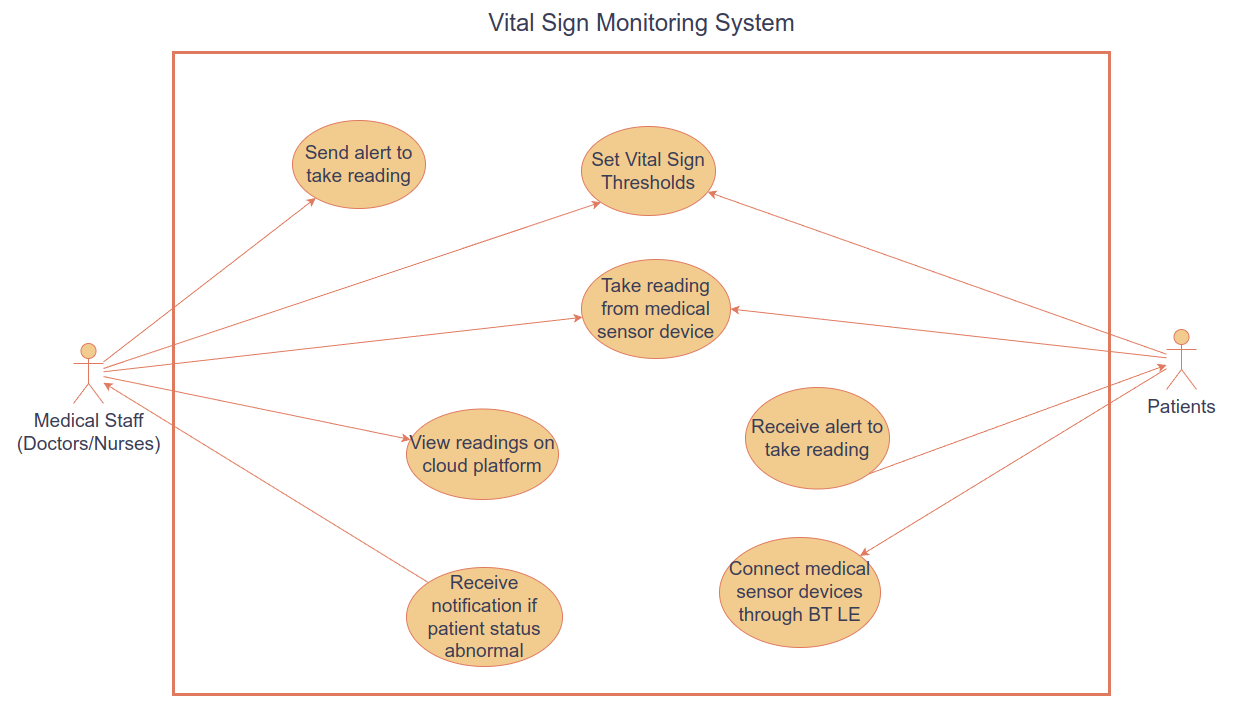
\includegraphics[width=\textwidth]{diagrams/use_case_diagram}
	\caption{Medical staff and patient interactions with the system}
	\label{fig:use_case_diagram}
\end{figure}

Following these exchanges, the system behaviour depicted in Figure \ref{fig:use_case_diagram} shows how the two user categories and the underlying monitoring functions are related. Every user role has a different workflow, as the diagram illustrates. Notably, the system will ask the patient to connect a compatible device and take the reading manually if medical staff requests a reading but there isn't a Bluetooth-connected medical sensor available at the moment. However, the use case diagram does not depict this internal fallback behaviour because these diagrams are meant to depict the actions that each actor can take that are visible to the outside world, not the internal logic or decision flows of the system. Nonetheless, this system ensures that clinical workflows are robust even when there are disconnections and that monitoring capability is maintained.

In conclusion, the system outlines the responsibilities of both patients and medical staff clearly, and takes into account situations where a reading is requested but there is no device connected to take it. Patients can also take readings throughout the day if they so desire, but when there is a remote request from a clinician it can not be ignored.

The system architecture and behavioural design, including state diagrams and the circuit diagram, are shown in the next section.

\section{System Architecture and Design} % Section 3.4
The architecture and design of the system are described in this section. For long-distance, low-power data transmission and centralised monitoring, the system includes a microcontroller-based LoRa communication unit. To gather data from the vital sign sensors, a Bluetooth Low Energy module is used, and for the communication between the device and the cloud a LoRaWAN gateway is set up to transmit to TheThingsNetwork. The goal of the design is to make it capable of communicating with BLE devices as simply as possible (something that due to the current closed nature of commerically available medical BT devices is not as simple as would be ideal), while utilising LoRaWAN's low-power features to allow for scalable, remote vital sign collecting, which is perfect for post-operative settings or locations with inadequate infrastructure.

Three main phases make up the system design: data collection (using the Bluetooth module to collect readings from medical sensors), processing of said data and finally transmission using an Arduino-based LoRa node. To tie everything together, cloud integration (using a LoRaWAN gateway and backend) will consist of a simple platform to view data and send commands to the device from a regular browser.

A high-level overview of the system's design is shown in Figure \ref{fig:high_level_architecture_diagram}. Blood pressure sensors, temperature sensors, and heart rate sensors are examples of medical Bluetooth capable devices that connect to a central unit (an Arduino-based microcontroller with a LoRa module) via Bluetooth LE. This central unit acts as a command centre and filter at the same time, where it filters out read data and only sends that which exceeds the set thresholds and is therefore considered critical data for a particular patient. It ignores data within bounds in all but a few cases --- those being when medical staff specifically request a reading, or the reading is one of those that are to be taken at set times every day.

This clearly compartmentalised architecture allows for separation of responsibilities: sensor management and handling of data is done locally, while the data is stored and analysed on the cloud platform. The cloud platform is also responsible for sending commands to the device when required by the medical staff.

\begin{figure}[H]
\centering
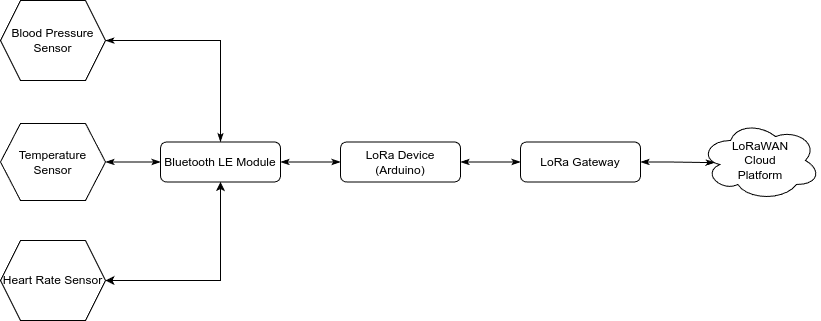
\includegraphics[width=\textwidth]{diagrams/high_level_architecture}
\caption{A high level view of the system architecture}
\label{fig:high_level_architecture_diagram}
\end{figure}

On the right side of Figure \ref{fig:high_level_architecture_diagram} is the LoRa Gateway which is responsible for bridging the device and the cloud platform.

The internal architecture of the embedded system is depicted in Figure \ref{fig:block_diagram}, which also highlights the hardware components' interactions on the Arduino-based microcontroller. The particular modules utilised in the finished implementation are shown in this diagram along with their functions in data collection, user interaction, processing, and communication.

\begin{figure}[H]
\centering
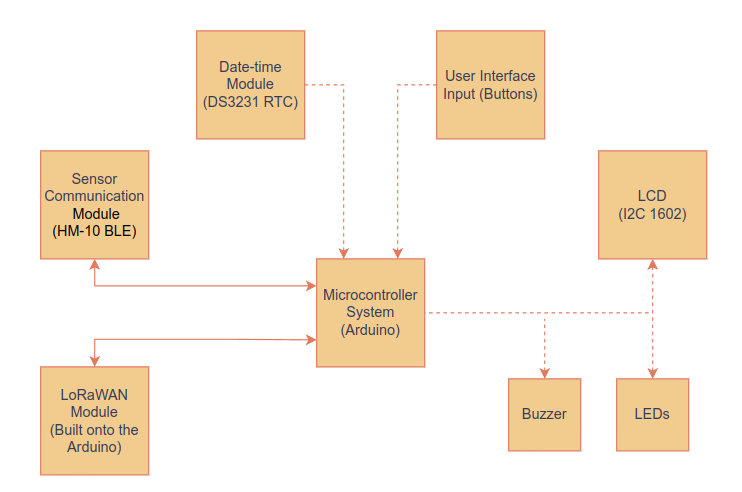
\includegraphics[width=\textwidth]{diagrams/block_diagram}
\caption{Block diagram showing relationships between high-level components of the system}
\label{fig:block_diagram}
\end{figure}

The core of the system is the Arduino microcontroller, which controls all data flow and peripheral interactions.

\begin{itemize}
	\item[] \textbf{Components for Sensing and Input}
	\item Module for Sensor Communication (HM-10 BLE): Communication with external medical devices, such as temperature, heart rate, and blood pressure sensors, is managed by this Bluetooth Low Energy module. This module is used by the Arduino to read data from the paired sensors.
	\item Date-Time Module: Accurate timestamps for sensor readings and intitiation of data reading at pre-programmed times of the day is provided by a real-time clock module (DS3231 RTC). This is crucial for monitoring vital sign trends over time. This data is read by the Arduino through I$^2$C.
	\item User Interface Input (Buttons): The patient can initiate actions, including entering reading mode and waiting for a reading or exploring menus on the display, by pressing buttons. This provides simple interaction without the need for additional devices.
	\item[] \textbf{Output and Feedback} 
	\item LCD Display: Shows timestamps, sensor data, and UI prompts in real time. This display uses very little GPIO thanks to the I$^2$C protocol.
	\item Local alarms are provided by the buzzer and the LEDs. System states, such as connected or disconnected, reading, processing, or errors can be represented by LEDs, and in the event of unusual readings or the need for user action, their attention can be grabbed by the use of the buzzer.
	\item[] \textbf{Transmission and Communication}
	\item LoRaWAN Module: This module manages wireless data transfer over great distances and is integrated into the Arduino board. After being taken and formatted, a reading is sent to the gateway via LoRa and uploaded to the cloud.
\end{itemize}

The system's behaviour can be varied based on the context and connected sensor thanks to its modular design using a Finite State Machine. Additionally, separated troubleshooting, streamlined development, and simpler future extensions (such incorporating SpO$_2$ sensors or supporting more sophisticated interfaces) are made possible by the separation of the communication, interface, and alarm modules. Next we will discuss the FSM that allows for this modularisation.

\subsubsection{State Machine Diagrams}
As soon as the system is turned on, it goes into the DISCONNECTED state. Awaiting user or environmental input, this state acts as the initial idle condition. In this state, two main conditions are assessed:

\begin{itemize}
	\item Without additional user interaction, the system switches straight to the CONNECTED state whenever a Bluetooth connection is discovered. When a compatible medical sensor is already activated and within range, this guarantees a smooth interaction.
	\item As an alternative, the system enters the SETUP state when the user chooses the "Setup" option from the interface, enabling the setting of vital sign thresholds before any sensors are connected.
\end{itemize}

\begin{figure}[H]
	\centering
	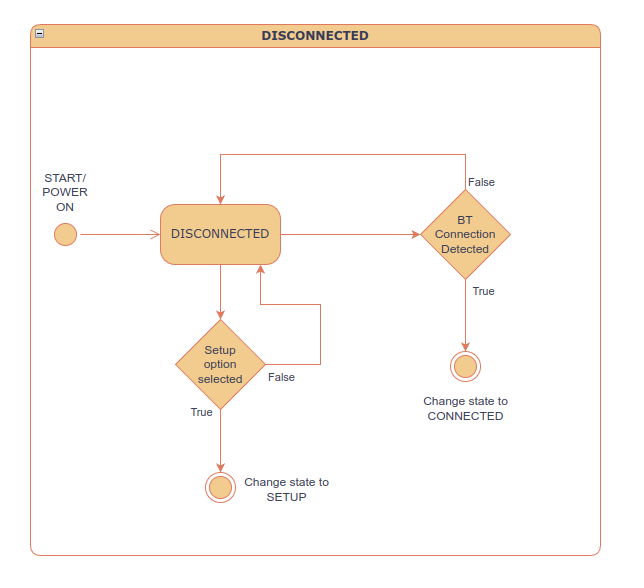
\includegraphics[width=\textwidth]{diagrams/states_disconnected}
	\caption{State diagram for the DISCONNECTED state}
	\label{fig:states_disconnected}
\end{figure}

Whether waiting for an automatic connection or permitting pre-configuration prior to active use, the decision structure guarantees flexibility and user-friendliness in the beginning stages of powering on (not requiring the user to explicitly enter the CONNECTED state if a device is already connected). The system can go on to measurement and data handling capability after configuration is finished or a device connects.

This flow can be seen visually represented as a state diagram in Figure \ref{fig:states_disconnected} above.

After a successful Bluetooth Low Energy (BLE) connection has been made with a medical sensor device, the CONNECTED state serves as the system's primary operating mode. In this condition, the user can take measurements or set up system parameters and has complete access to the system's essential features.

\begin{figure}[H]
	\centering
	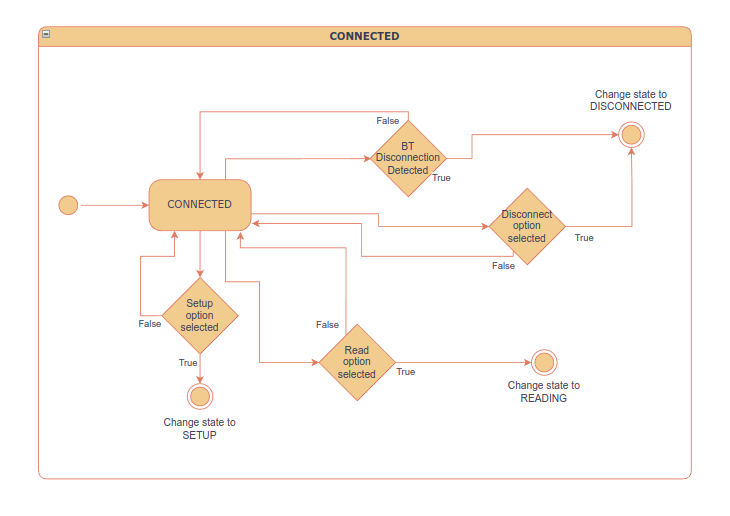
\includegraphics[width=\textwidth]{diagrams/states_connected}
	\caption{State diagram for the CONNECTED state}
	\label{fig:states_connected}
\end{figure}

The system offers three options from this state:

\begin{itemize}
	\item Setup: If the user selects the Setup option, the system enters the SETUP state, enabling the setup of vital sign thresholds.
	\item Read: Choosing the Read option puts the device in the READING mode and starts the process of gathering vital sign information from the linked medical sensor.
	\item Disconnect: The system returns to the DISCONNECTED state if the Disconnect option is chosen or if a Bluetooth disconnection is automatically detected. This guarantees that the availability of a linked sensor is always appropriately reflected by the system.
\end{itemize}

By ensuring that the system responds to user input as well as environmental changes (such a loss of connectivity), the state diagram preserves the system's resilience and user friendliness. Thus, the CONNECTED state acts as the centre for processes related to both configuration and data collection.

The interface for configuring the system's vital sign thresholds is accessible during the SETUP state. Depending on whether a Bluetooth-enabled sensor is currently coupled with the system, one can enter this state from either the DISCONNECTED or CONNECTED states.

\begin{figure}[H]
	\centering
	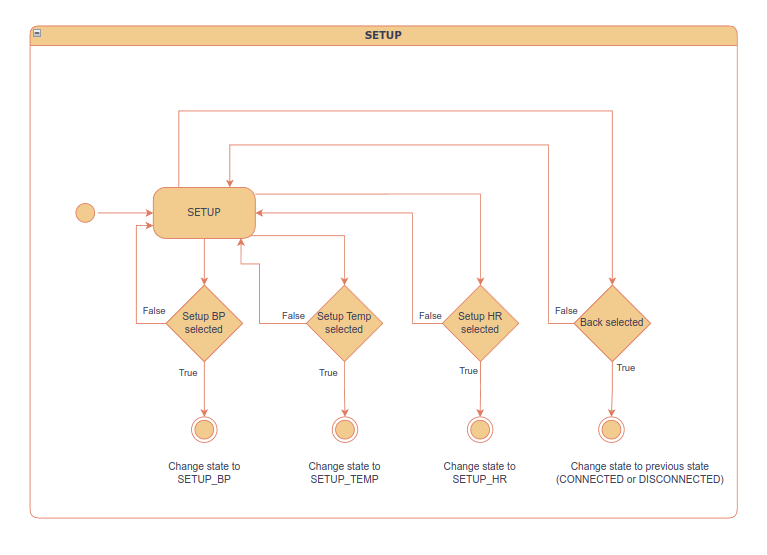
\includegraphics[width=\textwidth]{diagrams/states_setup}
	\caption{State diagram for the SETUP state}
	\label{fig:states_setup}
\end{figure}

As is visible from Figure \ref{fig:states_setup}, after entering the SETUP state, the user is given four options:

\begin{itemize}
	\item Setup BP (blood Pressure): This leads to the SETUP\_BP state, where the user can set the minimum and maximum systolic and diastolic thresholds accordingly.
	\item Setup Temp (Temperature): Allows the user to set the minimum and maximum temperature values by leading to the SETUP\_TEMP state.
	\item Setup HR (Heart Rate): This leads to the SETUP\_HR state where the user can set the minimum and maximum values for heart rate.
	\item Depending on where the SETUP state was called from, selecting the "Back" option will return the user to the CONNECTED or DISCONNECTED accordingly.
\end{itemize}

By serving as a routing hub, this state makes it possible to set clinical thresholds for each patient or surgery type. Each configuration option leads to a specific sub-state that handles validation and data entry logic; no threshold adjustments are made within this state itself.

The diagram below (Figure \ref{fig:states_setup_substates}) goes into detail for each of the setup sub-states.

\begin{figure}[H]
	\centering
	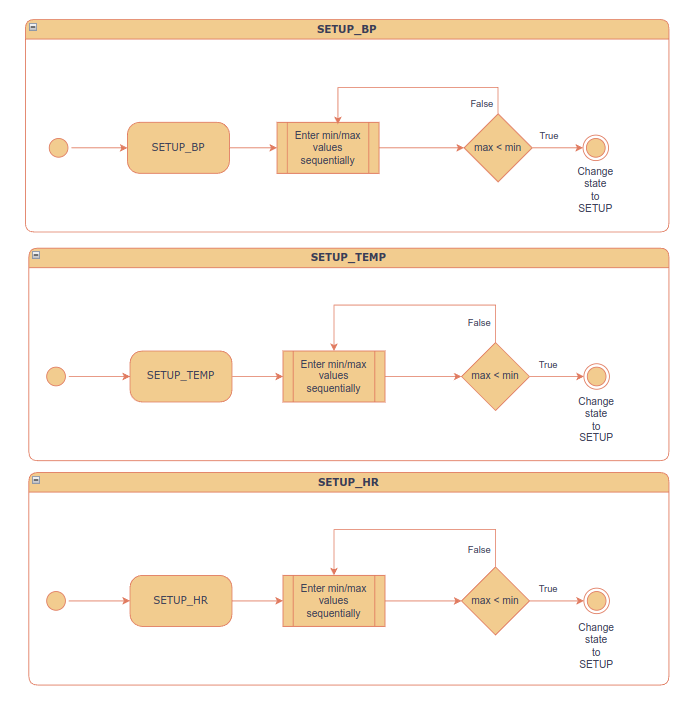
\includegraphics[width=\textwidth]{diagrams/states_setup_substates}
	\caption{State diagram for the SETUP sub-states}
	\label{fig:states_setup_substates}
\end{figure}

SETUP\_BP, SETUP\_TEMP, and SETUP\_HR are specifically responsible for setting the lowest and highest acceptable values for a given vital sign. The user is prompted to enter the values one after the other. To make sure the minimum is less than or equal to the maximum, each pair is separately checked. The system will re-prompt for both values if any validation is unsuccessful.

\begin{itemize}
	\item All of these states are essentially identical in structure and operation. They ask the user to enter a minimum and maximum value, check that the maximum is not less than the minimum, and if it is not return the user to the SETUP state.
\end{itemize}

These sub-states guarantee that threshold values used for measurement and analysis are reasonable, and enforce that thresholds are correctly set.

The READING state (Figure \ref{fig:states_reading}) is in charge of receiving vital sign information from a connected Bluetooth medical sensor. The system will wait for incoming data from the sensor device until something is received.

\begin{figure}[H]
	\centering
	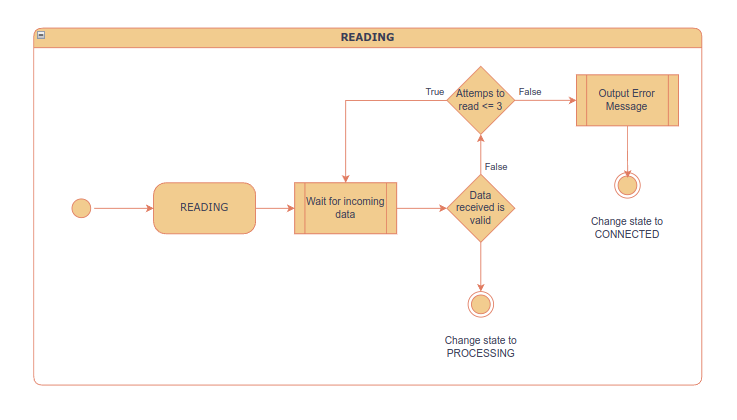
\includegraphics[width=\textwidth]{diagrams/states_reading}
	\caption{State diagram for the READING state}
	\label{fig:states_reading}
\end{figure}

Following the receipt of data, it must confirm that it's valid:

\begin{itemize}
	\item The system moves on to the PROCESSING state for more analysis if valid data is received.
	\item The system counts the number of read attempts if the data received is deemed invalid. Up to three attempts to read valid data are allowed.
	\item The system rejects the data and waits for a new reading if the number of attempts is less than or equal to three.
	\item The user is presented with an error message and the system returns to the CONNECTED state if the third attempt is unsuccessful as well.
\end{itemize}

The vital sign reading obtained in the previous READING state must be assessed by the PROCESSING state (Figure \ref{fig:states_processing}). The system determines if the newly received data is within the established acceptable bounds after it has been received. These thresholds, which are unique to each type of vital sign (e.g., blood pressure, heart rate, temperature), are established by the medical team or patient during system setup.

\begin{figure}[H]
	\centering
	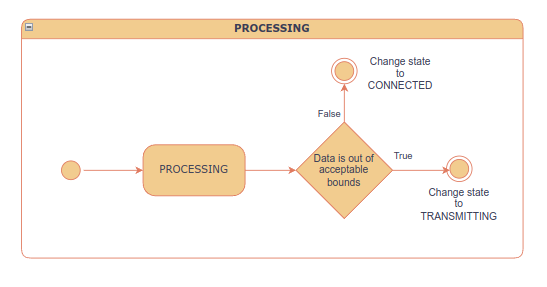
\includegraphics[width=\textwidth]{diagrams/states_processing}
	\caption{State diagram for the PROCESSING state}
	\label{fig:states_processing}
\end{figure}

The system returns to the CONNECTED state, where additional user input or new readings may be analysed, if the data falls within acceptable bounds and it decides that no immediate action is necessary. This is done to not flood the network with unnecessary traffic.

The data may, however, point to a potentially hazardous or abnormal patient condition if it drops below or goes above the established threshold range. The system then switches to the TRANSMITTING state, where it tries to transmit the abnormal reading to the cloud platform so that medical professionals can monitor it remotely.

This design ensures that alerts are raised only for clinically relevant events, reducing false alarms while maintaining responsiveness to potentially critical conditions, and reduces load on the network by only sending relevant data to the cloud.

Abnormal vital sign readings must be sent via LoRaWAN to the cloud platform while in the TRANSMITTING state (Figure \ref{fig:states_transmitting}). This only happens when a reading is outside the configured acceptable range, which indicates a possible health concern. This is determined by the PROCESSING state.

When the system reaches this state, the LoRa module on the Arduino starts the data transfer, after which it awaits confirmation from the cloud platform that the data was successfully received.

\begin{figure}[H]
	\centering
	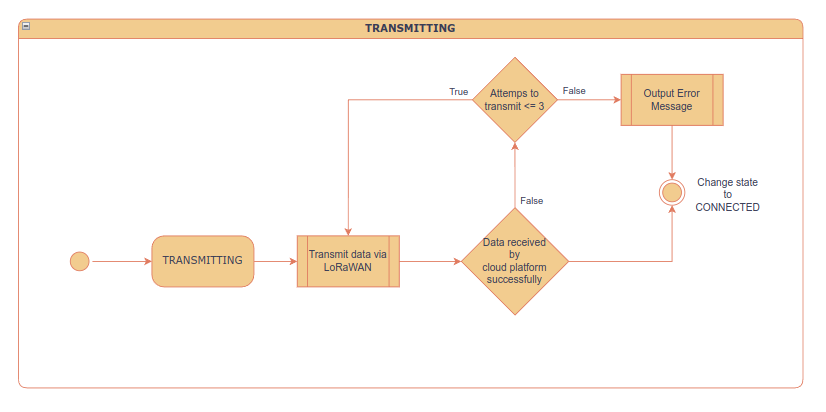
\includegraphics[width=\textwidth]{diagrams/states_transmitting}
	\caption{State diagram for the TRANSMITTING state}
	\label{fig:states_transmitting}
\end{figure}

Data transmission is deemed successful if confirmation is obtained in the form of an acknowledgement from the cloud platform, and the system goes back to the CONNECTED state, prepared to accept more inputs.

The system will attempt to deliver the data up to three times in the case of a failed transmission. The system notifies the user of the failure with an error message and returns to the CONNECTED state if, after three unsuccessful attempts, the data is still unable to reach the cloud platform. In addition to keeping the system from becoming permanently trapped in a failed state, this three-retries process helps guarantee reliability in wireless data transmission, particularly in settings where LoRaWAN connectivity may be erratic.

\subsubsection{Circuit Schematic}
The hardware circuit schematic for the system is displayed in Figure \ref{fig:circuit_diagram}. The system heart is the Arduino Leonardo microcontroller, which manages interfacing with peripheral components such the HM-10 Bluetooth Low Energy (BLE) module and the DS3231 real-time clock connected via I$^2$C. While the BLE module enables wireless connectivity to external sensor devices, the RTC maintains precise timekeeping for timestamping collected data, among other tasks.
The three-button interface allows for very basic user interaction in the form of menu navigation and threshold value entry. Four status LEDs—green, yellow, red, and blue—show the device's condition and Bluetooth connectivity. Additionally, a buzzer provides audible alerts for abnormal readings or transmission failures, and a 16x2 LCD display (as with the RTC, also connected via I$^2$C) is used to display menus. To guarantee a clear digital signal, a pull-down resistor is attached to each button, and 220 ohm resistors are used to limit the current flowing through all of the LEDs. This schematic represents a small, power-efficient design.
\begin{figure}[H]
\centering
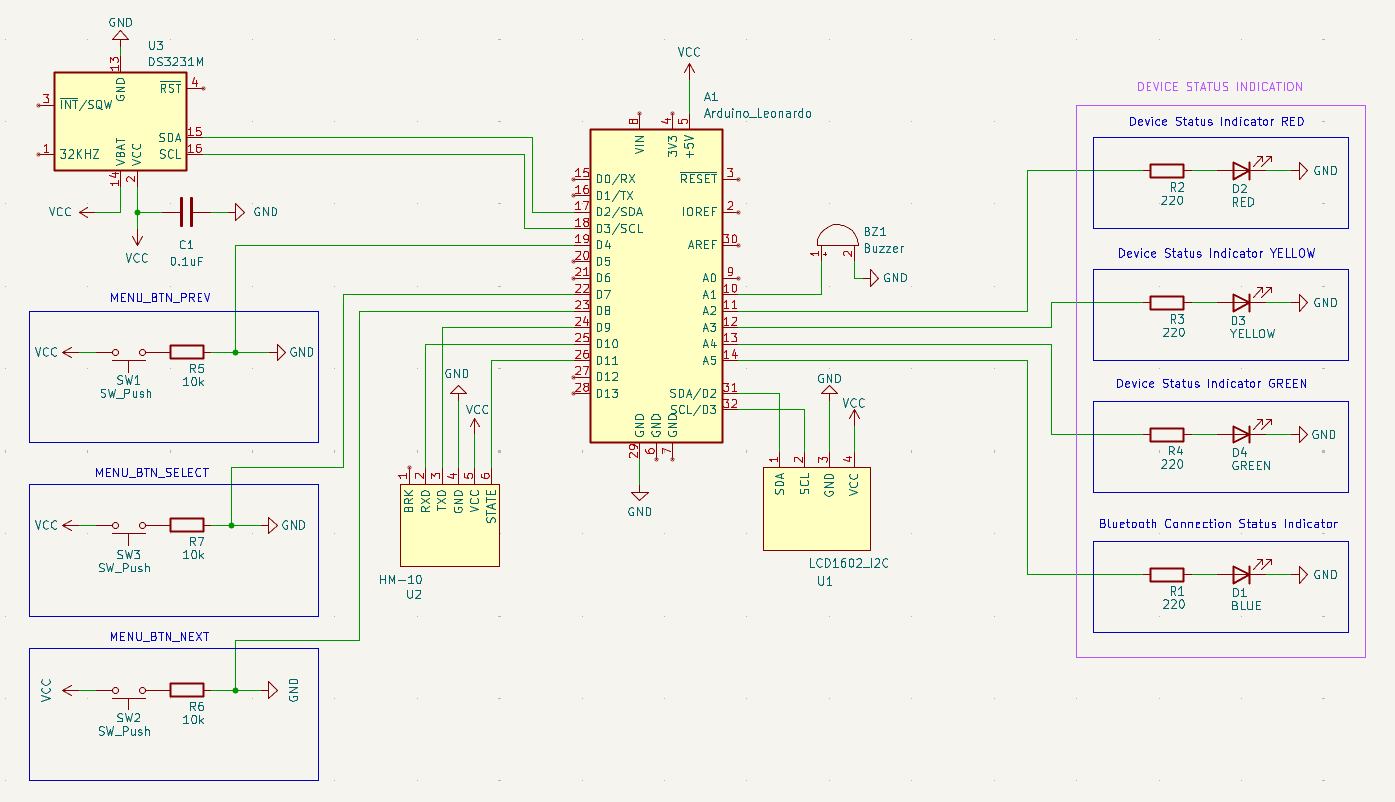
\includegraphics[width=\textwidth]{diagrams/schematic_rev3}
\caption{Detailed circuit shcemtatic of all all components in the device}
\label{fig:circuit_diagram}
\end{figure}

\section{User Interface Design} % Section 3.5
The device's user interface was made to be simple and easy to use, accommodating embedded technology limitations while guaranteeing medical staff and patients alike could easily interact with it. Push buttons, an LCD screen, a buzzer, and a group of LEDs make up the interface's four primary elements. Each one has a distinct function in communicating system status while occasionally their feedback cues may overlap to tell the user the same thing in different ways (e.g. Error displayed on the LCD while simultaneously a buzzer tone sounds corresponding to that error).

In addition to the device UI, there is the cloud dashboard UI, which I made using the TagoIO platform. It is split into four sections:
\begin{enumerate}
	\item \textbf{Commands:} This is where medical staff can send commands to the device such as a request for a reading or remote setting of vital sign thresholds (see Appendix~\ref{appendix:tagoio_commands}).
	\item \textbf{Blood Pressure:} This is where recevied blood pressure data can be visualised in two forms --- a vertical column view, and a line chart. (see Appendix~\ref{appendix:tagoio_bp})
	\item \textbf{Temperature:} This is where received temperature data can be visualised as a line chart. (see Appendix~\ref{appendix:tagoio_temp})
	\item \textbf{Heart Rate:} This is where received heart rate data can be visualised as a line chart. (see Appendix~\ref{appendix:tagoio_hr})
\end{enumerate}

Finally, I made a simple mobile app for testing purposes, to allow me to simply simulate medical sensors and their interactions with the system. The app's UI has four screens, with the main screen changing its appearance based on the connection status.
\begin{enumerate}
	\item \textbf{Main screen when first opening the app:} Contains an area to display simple logs, a button to clear the logs, and a button to start scanning for Bluetooth devices (see Appendix~\ref{appendix:app_ui_disconnected}).
	\item \textbf{Main screen when scanning for bluetooth devices:} When the button to start scanning is pressed, it changes to contain the text "Stop Scanning", and a list of available Bluetooth devices appears below it. When an item in the list is clicked, a connection is attempted to that device (see Appendix~\ref{appendix:app_ui_scanning})
	\item \textbf{Main screen when a connection has been established:} Contains an area to display logs, a button to disconnect the Bluetooth connection, and buttons to enter the screens for sending data to the device. (see Appendix~\ref{appendix:app_ui_connected}).
	\item \textbf{Screen for sending blood pressure data:} Contains an area to display simple logs, a back button, two text boxes to enter the systolic and diastolic values, and a button to send the data (see Appendix~\ref{appendix:app_ui_bp}).
	\item \textbf{Screen for sending temperature data:} Contains an area to display simple logs, a back button, a text boxe to enter the temperature value, and a button to send the data (see Appendix~\ref{appendix:app_ui_temp}).
	\item \textbf{Screen for sending heart rate data:} Contains an area to display simple logs, a back button, a text boxe to enter the heart rate value, and a button to send the data (see Appendix~\ref{appendix:app_ui_hr}).
\end{enumerate}

\subsubsection{Input Mechanism: Push Buttons}
Three push buttons are used by the system to facilitate option selection and menu navigation. These buttons are used to confirm selections and navigate through the available options (such as "Setup", "Read", or "Disconnect"). Only valid menu options are displayed at any given point thanks to the context-dependent functionality based on the current system state (as described in the state machine). Debouncing is handled in software to prevent unpredictable inputs.

\subsubsection{Visual Feedback: LCD Display}
A single 16x2 LCD module gives visual feedback to the user. This display, which shows menus, configuration options, and error alerts, acts as the primary means of communication between the user and the system. For instance, it shows any errors that may occur, or displays messages indicating to the patient that a request has come in from the cloud platform by a clinician. It is ideal for portable medical equipment due to its low power consumption, compact footprint, and microcontroller compatibility.

Below are examples of the two types of interactable menus. The first two are displayed when there is no active connection (Figure \ref{fig:ui_disconnected}) and when there is (Figure \ref{fig:ui_connected}), respectively, and demonstrate how the UI lets the user know that they can press the corresponding buttons to go left, right, or select the displayed option. The third image shows the menu displayed when setting the vital sign thresholds locally (Figure \ref{fig:ui_set_temp}). The difference between the set threshold menus and the regular ones is that in this one there are no options to cycle through, instead the vital sign being set is displayed (TEMP in this case) followed by the current value. The previous and next buttons now act as decrement/increment buttons, and this is conveyed to the user by adding a "-" and "+" symbol on the side of the corresponding buttons.

\begin{figure}[H]
	\centering
	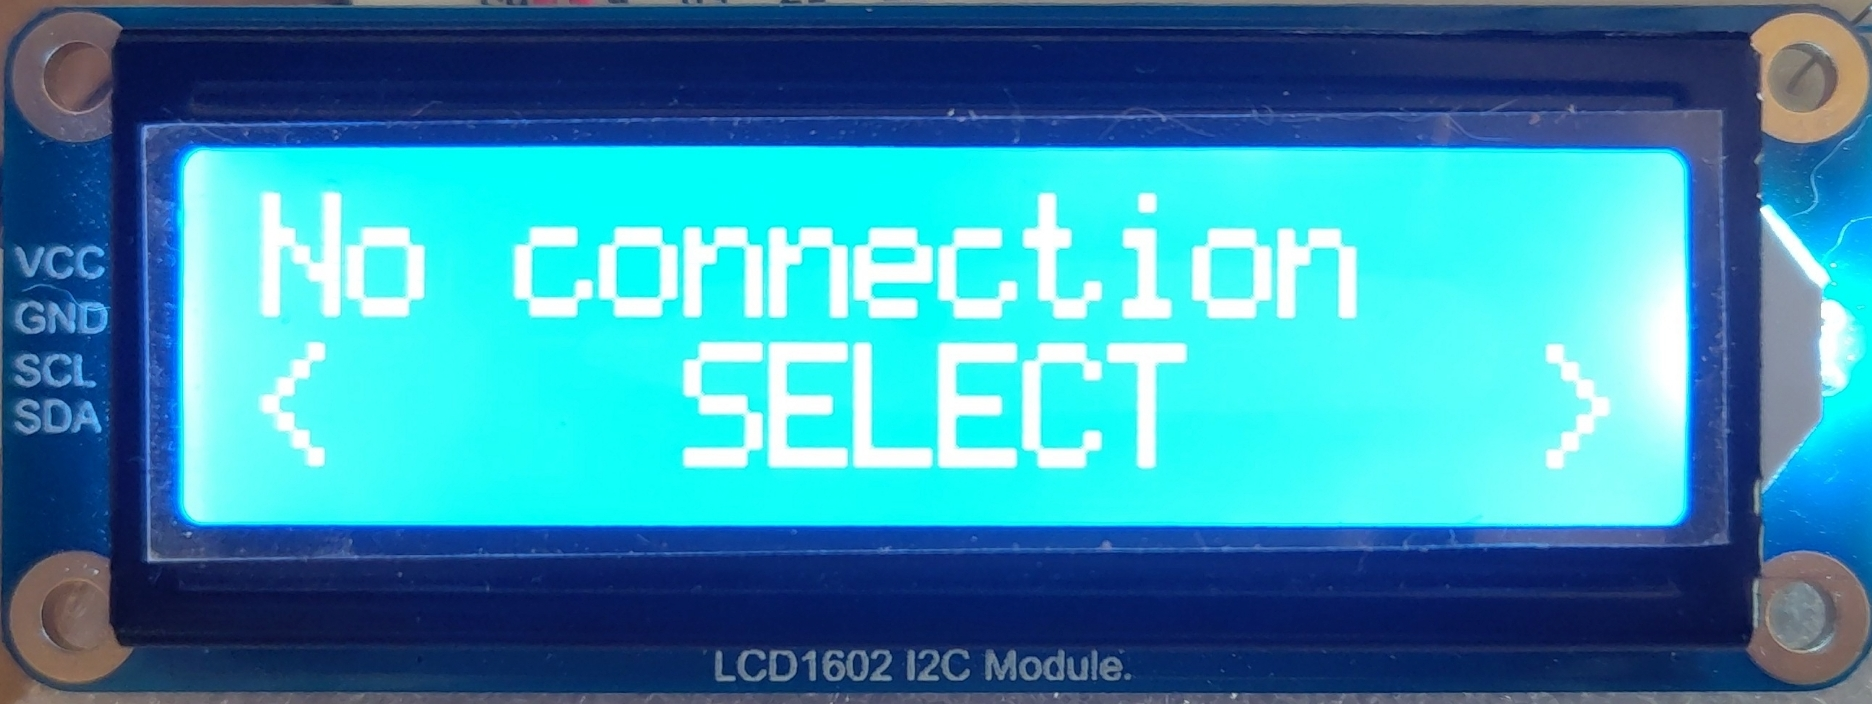
\includegraphics[width=0.55\textwidth]{images/device_ui_disconnected}
	\caption{Device UI when there are no active Bluetooth connections (see Appendix~\ref{appendix:ui_disconnected} for full size view)}
	\label{fig:ui_disconnected}
\end{figure}

\begin{figure}[H]
	\centering
	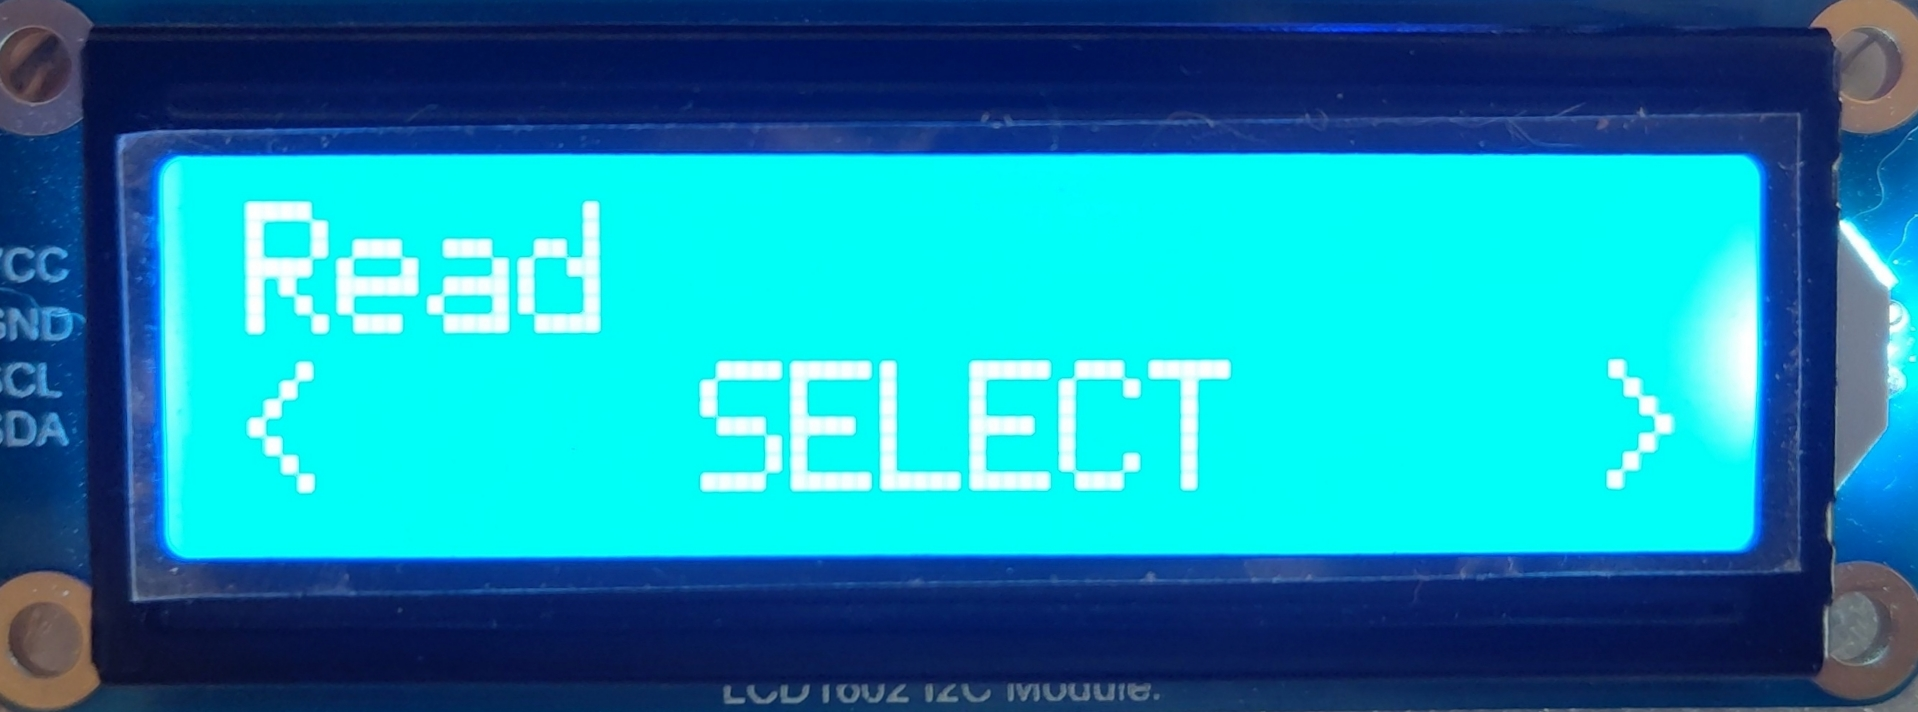
\includegraphics[width=0.55\textwidth]{images/device_ui_connected}
	\caption{Device UI when there are active Bluetooth connections (see Appendix~\ref{appendix:ui_connected} for full size view)}
	\label{fig:ui_connected}
\end{figure}

\begin{figure}[H]
	\centering
	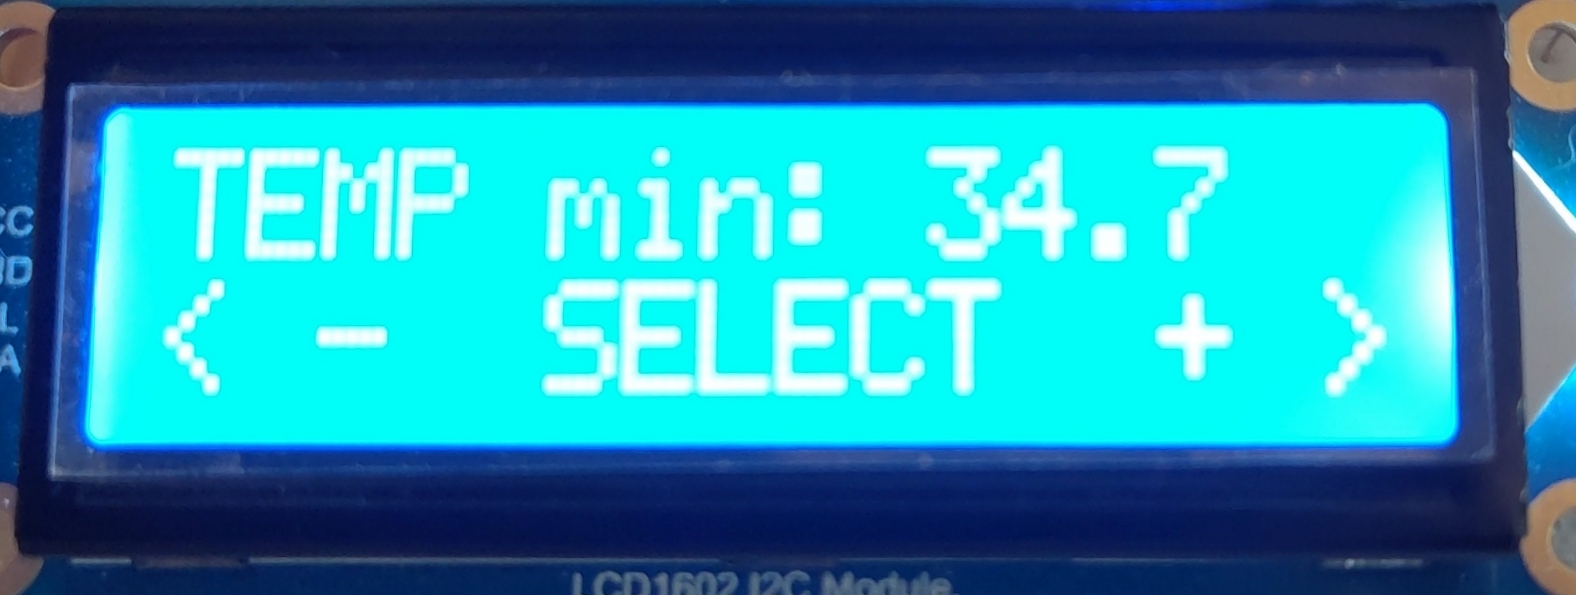
\includegraphics[width=0.55\textwidth]{images/device_ui_set_temp}
	\caption{Device UI when locally setting the temperature thresholds (see Appendix~\ref{appendix:ui_setup_temp} for full size view)}
	\label{fig:ui_set_temp}
\end{figure}

\subsubsection{Visual Feedback: Status Indicator LEDs}
Four LEDs are incorporated inside this device to give instantaneous, nonverbal feedback about connectivity and system status. Without looking at the LCD interface, users can rapidly determine operational conditions at a glance thanks to their clear and extremely simple nature. A different system state (not referring to states in the context of the state machine but rather operational conditions), such as regular operation, warnings, critical alerts, or connectivity status, is linked to each LED. By providing a quick overview of vital sign evaluations and device performance, this improves usability in clinical settings.

\subsubsection{Auditory Feedback: Buzzer}
Feedback is also provided by the buzzer on the device, for instance for abnormal measurements or any possible errors that may occur. For example, the buzzer emits certain tone patterns to notify either medical staff or the patient (if they have been released from hospital and are using the device for continuous at-home monitoring) if three consecutive read attempts are unsuccessful or if a vital sign reading deviates from permitted limits and must be transmitted. In situations where visual cues could be overlooked or are otherwise unavailable (e.g. if the patient is blind), the duality of having output both visually and audibly is vital.

The user interface design attempts to strike a balance between practicality and simplicity. It increases the system's dependability in a medical setting by reducing the need for user training and guaranteeing that important information is communicated quickly, while also providing the necessary functionality to control the system efficiently.

\section{Project Planning} % Section 3.6
To make sure that development, testing, and documentation progressed in a timely and systematic manner, the project execution was divided into distinct phases with some phases overlapping if it made sense to do so. The Gantt chart below shows the timeframe, which spans the months of October 2025 through May 2025. The pace and priority of the system's development and academic submission process are reflected in this timeline.

% \newgeometry{margin=1in}
\clearpage
\begin{landscape}
\vspace*{-1cm}
\begin{ganttchart}[
	hgrid,
	vgrid,
	time slot format=isodate-yearmonth,
	time slot unit=month,
	x unit=2.2cm,
	y unit chart=0.9cm,
	milestone label anchor/.append style={below=-1.6ex},
	milestone label font=\footnotesize\bfseries,
	bar label font=\normalsize\bfseries,
	bar/.append style={fill=blue!30},
	milestone/.append style={fill=red!70}
]{2024-10}{2025-05}

\gantttitlecalendar{year, month=shortname} \\

\ganttbar{Requirements Gathering}{2024-10}{2024-10} \\
\ganttbar{Literature Review}{2024-10}{2024-11} \\
\ganttbar{Hardware Design}{2024-12}{2025-04} \\
\ganttbar{Software Development}{2025-02}{2025-05} \\
\ganttbar{Thesis Writing}{2025-03}{2025-05} \\
\ganttbar{Testing and Debugging}{2025-04}{2025-05} \\
\ganttbar{Final Review \& Polish}{2025-05}{2025-05} \\
\ganttbar[bar/.append style={fill=green!70}]{Prototype Complete}{2025-05}{2025-05} \\
\ganttbar[bar/.append style={fill=blue!70}]{First Full Test}{2025-05}{2025-05} \\
\ganttbar[bar/.append style={fill=orange!60}]{Presentation}{2025-05}{2025-05} \\

\ganttnewline

\end{ganttchart}
\end{landscape}
\clearpage
% \restoregeometry


\begin{itemize}
	\item Gathering Requirements (October 2024): This initial phase concentrated on determining the system's objectives and functional requirements in light of postoperative care and Internet of Things-based medical monitoring.
	\item Review of Literature (October–November 2024): Research was done to comprehend the clinical and technical backdrop of vital sign monitoring systems, pertinent communication protocols, and medical device integration at the same time as requirements gathering.
	\item Hardware Design (December 2024–April 2025): This stage included choosing and integrating sensors, microcontrollers, and communication modules as well as designing and developing the device's electronics and circuit-level architecture.
	\item Software Development (February-May 2025): This stage, which overlapped with hardware design, concentrated on developing the Arduino-based system's firmware, putting state logic into practice, and providing preliminary support for receiving and transmitting sensor data.
	\item Thesis Writing (March–May 2025): As development stabilised, the thesis's composition and writing got underway. This made it possible to provide actual implementation information, system schematics, and assessment findings.
	\item Testing and Debugging (April–May 2025): This step involved testing system module integration, validating state transitions, and improving threshold configuration and error-handling procedures all at the same time as documentation.
	\item Thesis Final Evaluation and Polishing (May 2025): With the help of my supervisors, revisions were made to the thesis, and mistakes corrected.
	\item First complete version finalised (May 2025): First completely working version done and ready for full testing.
	\item Presentation (May 2025): Visual aids and practice sessions for the project's final presentation.
\end{itemize}

\section{Summary} % Section 3.7
This section described the full foundational design of the system being developed, starting with an assessment of the user and technical requirements. These served as a guide for overall development and were drawn from the practical demands of postoperative patient care.

The interactions between patients, medical personnel, and the system were made clear by the use case diagram. This section also highlighted the ways in which data is gathered, sent, and examined. The architecture of the system, including high-level data flow and hardware integration, was discussed introducing the main technological elements such as the LoRaWAN communication backbone and the microcontroller-based circuit architecture. Following that, the user interface design was discuseed in detail, analysing the function and reasoning behind the LEDs, the LCD screen, the buttons, and the buzzer. The project's development cycle was finally depicted by a Gantt chart, which demonstrated how the many design and implementation phases were arranged and overlapped to effectively fulfil deadlines. When combined, these components create a coherent and well-designed system that meets the specified technological and practical objectives while retaining extensibility and adaptability for future modifications.
